\section{Background}
\subsection{Itemset mining for decision trees}
We limit our discussion to the key ideas behind DL8, and assume that the reader is already familiar with the general concepts behind learning decision trees.

DL8 operates on Boolean data. As running example of such data, we will use the dataset of Table 1a, which consists of three Boolean features and eleven examples. The optimal decision tree for this database can be found in Figure 1a. While it may seem a limitation that DL8 only operates on Boolean data, there are straightforward ways to transform any tabular database in a Boolean database: for categorical attributes, we can create a Boolean column for each possible value of that attribute; for numerical attributes, we can create Boolean columns for possible thresholds for that attribute.

DL8 takes an itemset mining perspective on learning decision trees. In this perspective, the binary matrix of Table \ref{tab:1a} is transformed into the transactional database of Table \ref{tab:1b}. Each transaction of the dataset contains an itemset describing the presence or absence of each feature in the dataset. More formally, the database $\mathcal{D}$ can be thought of as a collection $\mathcal{D} = \{(t, I, c)\;|t\in \mathcal{T} , I \subseteq \mathcal{I}, c \in \mathcal{C}\}$, where $\mathcal{T}$ represents the transaction or rows identifiers, $\mathcal{I}$ is the set of possible items, and $\mathcal{T}$ is the set of class labels; within $\mathcal{I}$ there are two items (one positive, the other negative) for each original Boolean feature, and each itemset $I$ contains either a positive or a negative item for every feature.
\begin{table}[!ht]
	\centering
	\subfloat[Binary matrix\label{tab:1a}]{
		\begin{tabular}{c|c|c||c}
			\hline
			A		&	B	&	C	&	classe		\\
			\hline
			0		&	1	&	1	&	0			\\
			1		&	0	&	1	&	1			\\
			0		&	0	&	1	&	1			\\
			0		&	1	&	0	&	0			\\
			1		&	0	&	0	&	1			\\
			0		&	0	&	0	&	0			\\
			0		&	0	&	1	&	0			\\
			1		&	1	&	0	&	1			\\
			0		&	0	&	0	&	1			\\
			0		&	0	&	1	&	0			\\
			0		&	0	&	0	&	1			\\
			\hline
		\end{tabular}
	}~
	\subfloat[Transactional database\label{tab:1b}]{
		\begin{tabular}{c||c||c}
			\hline
			rowId	&	items		&	class	\\
			\hline
			1		& $¬a, b, c$	&	0		\\
			2		& $a, ¬b, c$	&	1		\\
			3		& $¬a, ¬b, c$	&	1		\\
			4		& $¬a, b, ¬c$	&	0		\\
			5		& $a, ¬b, ¬c$	&	1		\\
			6		& $¬a, ¬b, ¬c$	&	0		\\
			7		& $¬a, ¬b, c$	&	0		\\
			8		& $a, b, ¬c$	&	1		\\
			9		& $¬a, ¬b, ¬c$	&	1		\\
			10		& $¬a, ¬b, c$	&	0		\\
			11		& $¬a, ¬b, ¬c$	&	1		\\
			\hline
		\end{tabular}
	}
	\caption{Example database}
	\label{tab:1}
\end{table}

\begin{figure}
	\centering
	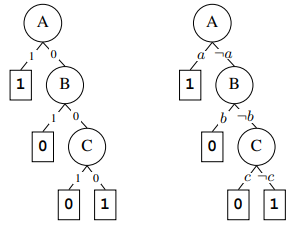
\includegraphics[width=0.79\linewidth]{graph}
	\caption{Optimal tree corresponding to database of Table \ref{tab:1}. Max depth = 3 and minimum examples per leaf = 1}
	\label{fig:1}
\end{figure}
Using this representation, every path in a decision tree can be mapped to an itemset $I \subseteq \mathcal{I}$, as shown in Figure \ref{fig:1b}. For instance, the last path in this tree corresponds to the itemset $\{\neg a, \neg b, \neg c\}$. Please note that multiple paths can be mapped
to the same itemset.

For every itemset $I$, we define its cover to be $cover (I) = \{(t', I' , c') \in \mathcal{D} | I \subseteq I'\}$ : the set of transactions in which the itemset is contained; the class-based support of an itemset is defined as $Sup(I, c) = |\{(t', I', c')\in cover (I)| c' = c\}|$, and can be used to identify the number of examples for a given class c in a leaf. Based on class-based supports, the error of an itemset is defined as:
\begin{equation}
	leaf\_error(I) =| cover(I) | - \max_{c\in\mathcal{C}}\{Sup(I,c)\}
	\label{eq:1}
\end{equation}

Unlike the CP-based approach, our error function is also valid for classification tasks involving more than 2 classes.

The canonical decision tree learning problem that we
study in this work can now be defined as follows using itemset mining notation. Given a database $\mathcal{D}$, we wish to identify a collection $\mathcal{DT} \subseteq \mathcal{I}$ of itemsets such that
\begin{itemize}
	\item the itemsets in DT represent a decision tree;
	\item $\sum_{I\in\mathcal{DT}} leaf\_error(I)$ is minimal;
	\item for all $I\in\mathcal{DT} : |I| \le maxdepth$, where $maxdepth$ is the maximum depth of the tree;
	\item for all $I\in\mathcal{DT} :| cover(I) \ge minsup$, where $minsup$ is a minimum support threshold.
\end{itemize}
As stated earlier, in DL8, the maximum depth constraint is not required; MIP-based approaches have ignored the minimum support constraint.
